\documentclass[14pt]{beamer}
\usetheme{Boadilla}

\usepackage[utf8]{inputenc}
\usepackage[T1]{fontenc}
\usepackage[portuguese]{babel}
\usepackage{booktabs}
\usepackage{lmodern}
\usepackage{listings}
\lstset{
	basicstyle=\scriptsize\ttfamily,
	numbers=left,
	numberstyle=\tiny,
	numbersep=5pt,
	frame=single
}
\renewcommand{\arraystretch}{1.2}

\title[eProfile]{Um Modelo para Gerenciamento de Perfis de Entidades Através de Inferência em Trilhas}
\author[André Wagner]{André Wagner\\{\small Orientador: Dr. Jorge Luis Victória Barbosa}}
\institute[UNISINOS]{
  Programa de Pós-Graduação em Computação Aplicada \\
  Universidade do Vale do Rio dos Sinos (UNISINOS) \\
  \texttt{andre.nho@gmail.com}
}

\begin{document}

%%%

\begin{frame}[plain]
  \titlepage
\end{frame}

%%%

\begin{frame}
  \frametitle{Organização}
  \begin{enumerate}
    \item Introdução
    \item Modelo
    \item Implementação
    \item Avaliação
    \item Conclusão
  \end{enumerate}
\end{frame}

%%%

\begin{frame}
  \huge Introdução
\end{frame}

%%%

\begin{frame}
  \frametitle{Computação Ubíqua}
  \begin{itemize}
    \item Tendências da computação
    \begin{itemize}
      \item Computadores cada vez menores e mais rápidos
      \item Componentes cada vez mais baratos
      \item Acesso a redes {\em wireless} cada vez mais disponível
    \end{itemize}
    \item Serviços computacionais disponíveis a todo momento em qualquer lugar
    \item Tecnologia Calma
    \begin{itemize}
      \item Problema: sobrecarga de informações para o usuário
      \item Solução: sistemas minimamente intrusivos
      \item ``Periferia'' da atenção do usuário
      \item Exemplo: motor de carro
    \end{itemize}
  \end{itemize}
\end{frame}

%%%%%

\begin{frame}
  \frametitle{Contexto}
  \begin{itemize}
    \item Para que um sistema seja minimamente intrusivo
    \begin{itemize}
      \item Conhecer o usuário
      \item Conhecer os arredores do usuário
      \item Adaptar-se a esta informação
    \end{itemize}
    \item {\bf O que é contexto?}
    \begin{itemize}
      \item ``Contexto é qualquer informação que possa ser usada para 
      caracterizar a situação de uma entidade. Uma entidade é uma pessoa, 
      local ou objeto que seja considerada relevante para a interação entre 
      um usuário e uma aplicação, incluindo o próprio usuário e aplicação.'' (Dey, 2001)
    \end{itemize}
  \end{itemize}
\end{frame}
    
%%%%%

\begin{frame}
  \frametitle{Trilhas}
  \begin{itemize}
    \item Contexto é composto apenas pelo momento atual
    \item A capacidade de uma aplicação compreender o contexto de uma entidade pode ser ampliada através da análise dos históricos.
    \item Uma \textbf{trilha} é o histórico de contextos visitados por uma entidade e das ações realizadas pela entidade dentro do contexto
  \end{itemize}
\end{frame}
    
%%%%%

\begin{frame}
  \frametitle{Perfis}
    \begin{itemize}
      \item Este trabalho usa o conceito de \textbf{entidade} ao invés de usuário.
      \item \textbf{Perfis} são essenciais na descoberta de informações pertinentes às entidades que possam ser utilizadas na construção de um contexto.
      \item Um \textbf{perfil de entidade} é o conjunto de dados no qual uma aplicação armazena seu conhecimento a respeito de uma entidade. 
      \item Os perfis de entidade são salvos em um formato chamado \textbf{modelo de entidade}.
    \end{itemize}
\end{frame}
    
%%%%%

\begin{frame}
  \frametitle{Interoperabilidade}
  \textbf{Interoperabilidade} é a capacidade de dois ou mais sistemas ou componentes trocarem informações e utilizar a informação que foi trocada.
  \begin{itemize}
    \item Modelos de Interoperabilidade
    \begin{description}
      \item[Sintática:] diferenças entre os modelos de usuário são resolvidos em nível de aplicação.
      \item[Semântica:] diferenças entre os modelos são resolvidos em nível de conhecimento.
    \end{description}
  \end{itemize}
\end{frame}
    
%%%%%%%%%%%%%%%%%%%%%%

\begin{frame}{Trabalhos relacionados}

	\begin{table}\centering\fontsize{7}{13}\selectfont
  \begin{tabular*}{1\textwidth}{@{}llllllllll@{}}
    \toprule
    			      & PeLeP    & Chellouche & UUCM      & Kim       & Razmerita & Tao \\
    \midrule
    Interoperabilidade        & Não      & Sintática  & Sintática & Sintática & Sintática & Semântica \\
    Modelos dinâmicos         & Não      & Não        & Não       & Não       & Não       & Não \\
    Armazenamento             & Servidor & Servidor   & Cliente   & Servidor  & Servidor  & Servidor \\
    Sensibilidade a contexto  & Sim      & Sim        & Sim       & Não       & Sim & Sim \\
    Utiliza trilhas           & Parcial  & Não        & Não       & Parcial   & Parcial   & Parcial \\
    Domínio                   & Educação & Multimídia & Genérico  & Genérico  & Genérico  & Genérico \\
    \bottomrule
  \end{tabular*}
  \caption{Comparação entre os trabalhos apresentados}
  \label{tab:comparacao}
\end{table}

\end{frame}

%%%%%

\begin{frame}
  \frametitle{Problema de Pesquisa}
  \begin{itemize}
    \item Geração de perfis dinâmicos
    \item Uso de trilhas para extração de perfis
    \item Domínio genérico
    \item Regras de inferência e modelos de entidades dinâmicos
    \item Interoperabilidade semântica
  \end{itemize}
\end{frame}

%%%

\begin{frame}
  \huge Modelo
\end{frame}

%%%%%

\begin{frame}
  \frametitle{eProfile}
\textbf{eProfile}: um \textcolor{blue}{gerenciador de perfis} de \textcolor{blue}{domínio genérico} voltado para \textcolor{blue}{ambientes distribuídos}, com \textcolor{blue}{interoperabilidade inter-sistemas}, que \textcolor{blue}{infere dados de perfil} através da \textcolor{blue}{análise das trilhas} de uma entidade (disponibilizadas por um gerenciador de trilhas), seguindo \textcolor{blue}{regras definidas pelas entidades}, e \textcolor{blue}{disponibiliza os dados} inferidos para serem utilizados pelas aplicações.
\end{frame}

%%%%%

\begin{frame}
  \frametitle{Modelo do eProfile}
\begin{figure}
  \centering
\includegraphics[width=0.7\textwidth]{../imagens/modelobasico.png}
  \caption{Modelo básico do eProfile}
\end{figure}
As setas representam o fluxo dos dados.
\end{frame}


%%%%%

\begin{frame}
  \frametitle{Modelo do eProfile}
\begin{figure}
  \centering
\includegraphics[width=0.7\textwidth]{../imagens/modelo2.png}
  \caption{eProfile conectado a mais de um gerenciador de trilhas}
\end{figure}
\end{frame}

%%%%%

\begin{frame}
  \frametitle{Modelo do eProfile}
\begin{figure}
  \centering
\includegraphics[width=0.9\textwidth]{../imagens/modelo.png}
  \caption{Modelo simplificado do eProfile}
\end{figure}

\end{frame}

%%%%%

\begin{frame}
  \frametitle{Ontologias}
  \begin{itemize}
    \item Extensível
    \item Linguagem utilizada: OWL (extensão de XML/RDF)
  \end{itemize}
  Ontologias do eProfile
  \begin{itemize}
    \item eOntoTrail: representação de trilhas
    \item eOntoProfile: representação de perfis
  \end{itemize}
\end{frame}

%%%%%

\begin{frame}
  \frametitle{Ontologia de Trilha}
\begin{figure}
  \centering
\includegraphics[width=1\textwidth]{../imagens/ont_trilha_simples.png}
  \caption{Ontologia de Trilha do eProfile}
\end{figure}
  
\end{frame}

%%%%%

\begin{frame}
  \frametitle{Ontologia de Perfis}
\begin{figure}
  \centering
\includegraphics[width=0.8\textwidth]{../imagens/ont_perfil2.png}
  \caption{Ontologia de Perfil do eProfile}
\end{figure}

\end{frame}

%%%%%

\begin{frame}
  \frametitle{Regras}
  \begin{itemize}
    \item Regras:
    \begin{itemize}
      \item OWL
      \item SPARQL (consulta) 
      \item SWRL (lógica)
    \end{itemize}
    \item Uma regra possui as seguintes informações:
    \begin{itemize}
      \item Nome
      \item Campo de perfil
      \item Regra
      \item Atualização (sobrescrito/fórmula)
      \item Frequência de atualização
      \item Validade
    \end{itemize}
  \end{itemize}
\end{frame}

%%%%%%%%%%

\begin{frame}
  \frametitle{Exemplo}
  
  \begin{itemize}
    \item Curso de programação em linguagens orientadas a objeto
    \item Aluno estuda através de dispositivo móvel
    \item Para fazer a prova final, o aluno deve ter concluído os módulos daquela linguagem
  \end{itemize}

  \begin{figure}
    \centering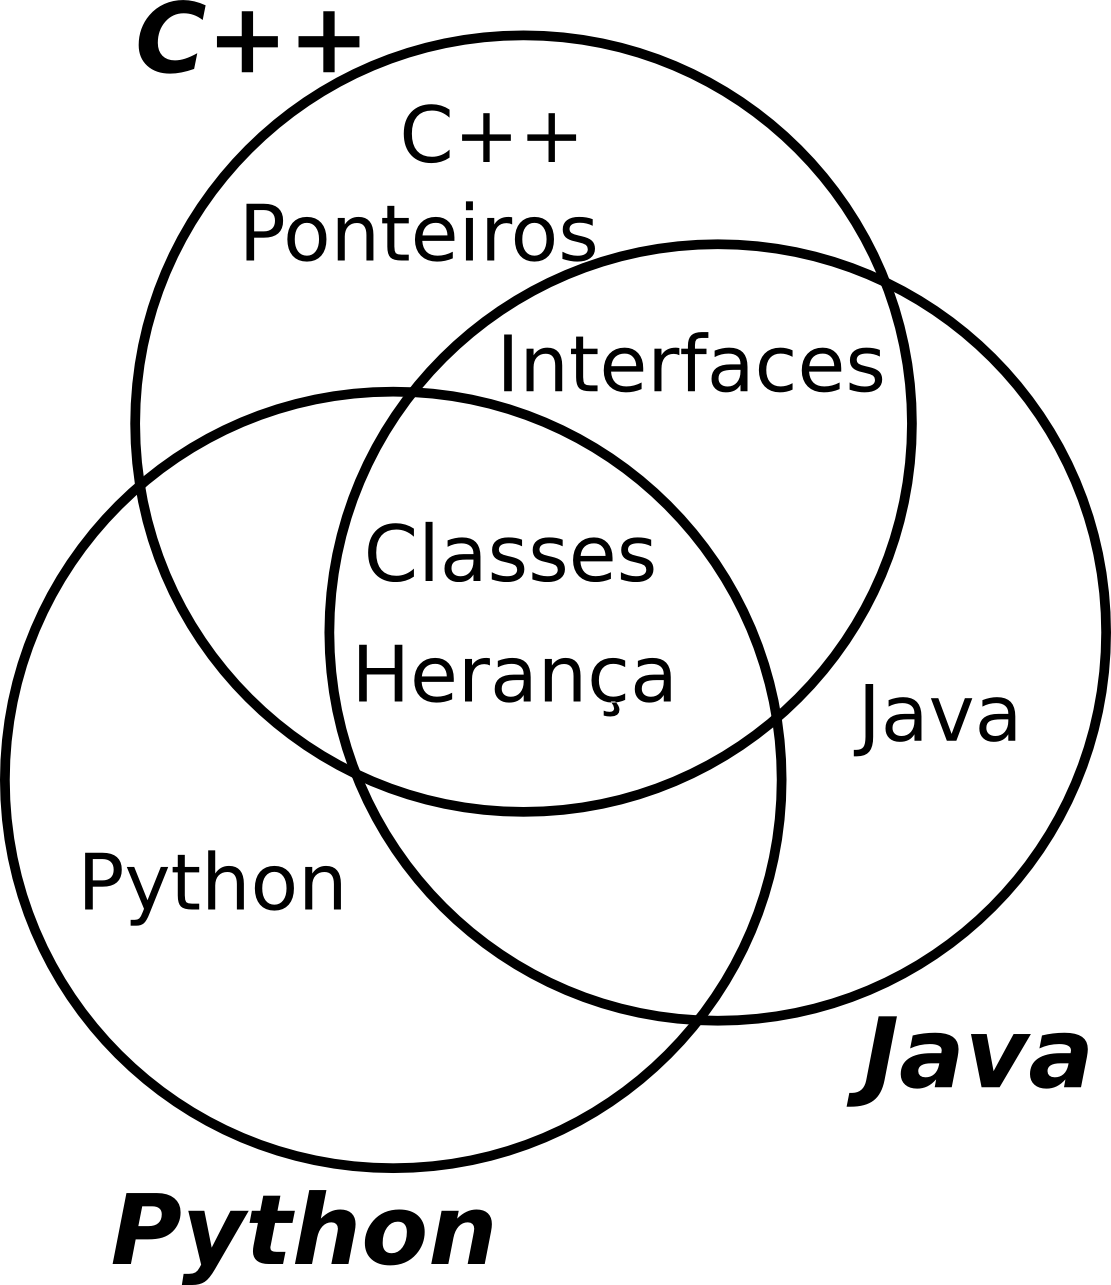
\includegraphics[width=0.25\textwidth]{../imagens/cen1_modulos.png}
    \caption{Módulos de estudo obrigatórios}
  \end{figure}

\end{frame}

%%%%%

\begin{frame}
  \frametitle{Exemplo}
  
  \begin{figure}
    \centering
\includegraphics[width=0.9\textwidth]{../imagens/cen_ontologia.png}
    \caption{Informações contextuais}
  \end{figure}
\end{frame}

%%%%%

\begin{frame}[fragile]
  \frametitle{Exemplo - Regras}
 
\begin{lstlisting}
Class: <el:JavaRequirement>
    EquivalentTo: 
        <el:Java>
         or (<el:relatesTo> some <el:Java>)

Class: <el:JavaLessonsTaken>
    EquivalentTo: 
        <el:FinishedLOEvent>
         and (<el:hasEntity> some [?entity])
         and (<el:hasLearningObject> some 
	                        <el:JavaRequirement>)
         and (<el:isFirstTime> value true)

JavaProficience <= 
  (Count(SubClasses(JavaRequirement))) equals
          (Count(SubClasses(JavaLessonsTaken)))
\end{lstlisting}

\end{frame}

%%%%%

\begin{frame}[fragile]
  \frametitle{Exemplo - Definição da Regra}
\begin{lstlisting}
Entity:    Student
Field:     Knowledge\JavaProficience
Rule:      JavaProficience
Update:    update
Frequence: 300
Expires:   never
\end{lstlisting}
  
\end{frame}

%%%%%

\begin{frame}[fragile]
  \frametitle{Exemplo - Perfil Gerado}
\begin{lstlisting}
Ontology: <el>

Class: <el:Knowledge>

Class: <el:JavaProficience>
    SubClassOf: 
        <el:Knowledge>
ObjectProperty: <el:hasKnowledge>
    
Class: <el:Entity>
    
Class: <el:Maria>
    SubClassOf: 
        <el:Entity>
    
Class: <el:Andre>
    SubClassOf: 
        <el:Entity>,
        <el:hasKnowledge> some <el:JavaProficience>
\end{lstlisting}
  
\end{frame}

%%%

\begin{frame}
  \huge Implementação
\end{frame}

%%%%%

\begin{frame}
  \frametitle{Implementação - Tecnologias Utilizadas}
  \begin{itemize}
    \item Linguagem de programação: {\bf Python}
    \item Banco de dados: {\bf SQLite3}
    \item Aplicativos contectados via {\bf {\em webservices} do tipo REST}
    \item Motor de inferência: {\bf FaCT++}
    \item Linguagem de ontologia: {\bf OWL DL}
  \end{itemize}
  
\end{frame}

%%%%%

\begin{frame}
  \frametitle{Implementação}
  \begin{figure}
    
\includegraphics[width=1\textwidth]{../imagens/classes.png}
    \caption{Diagrama de classes}
  \end{figure}
  
\end{frame}

%%%%%

\begin{frame}
\begin{figure}
  
\includegraphics[width=0.65\textwidth]{../imagens/activity.png}
  \caption{Diagrama de sequência}
\end{figure}
  
\end{frame}

%%%

\begin{frame}
  \huge Avaliação
\end{frame}

%%%%%

\begin{frame}
  \frametitle{Cenário}
  \begin{itemize}
    \item Simulação de um curso de ciência da computação
    \item 40 disciplinas
    \item Ambiente de Educação Ubíqua
    \item Integração com sistemas: 
      \begin{itemize}
        \item LOCAL: sistema de educação ubíqua que usa informações de localização e contexto para auxiliar o processo de apendizagem
        \item UniManager: software administrativo da universidade, controla presenças e matrículas
      \end{itemize}
  \end{itemize}
  
\end{frame}

%%%%%

\begin{frame}
  \frametitle{Cenário}
  \begin{itemize}
    \item Alterações feitas no LOCAL e no UniManager:
      \begin{itemize}
        \item Incluídas {\em interfaces} de comunicação com o eProfile
        \item Incluídas {\em interfaces} de comunicação com o Gerenciador de Trilhas 
        \item O módulo de perfis de ambas as aplicações foi modificado de modo a solicitar as atualizações de perfil a partir do eProfile
      \end{itemize}
    \item Simuladores
      \begin{itemize}
        \item Simluação dos estudantes e docentes
        \item Gerenciador de trilhas simulado
      \end{itemize}
  \end{itemize}
  
\end{frame}

%%%%%

\begin{frame}
  \frametitle{Cenário}
  \begin{figure}
    \centering
    
\includegraphics[width=0.8\textwidth]{../imagens/modelo_cenario1.png}
    \caption{Modelo do Cenário}
  \end{figure}
  
\end{frame}

%%%%%

\begin{frame}
  \frametitle{Cenário - Integração eProfile/LOCAL}
  \begin{figure}[!t]
    \centering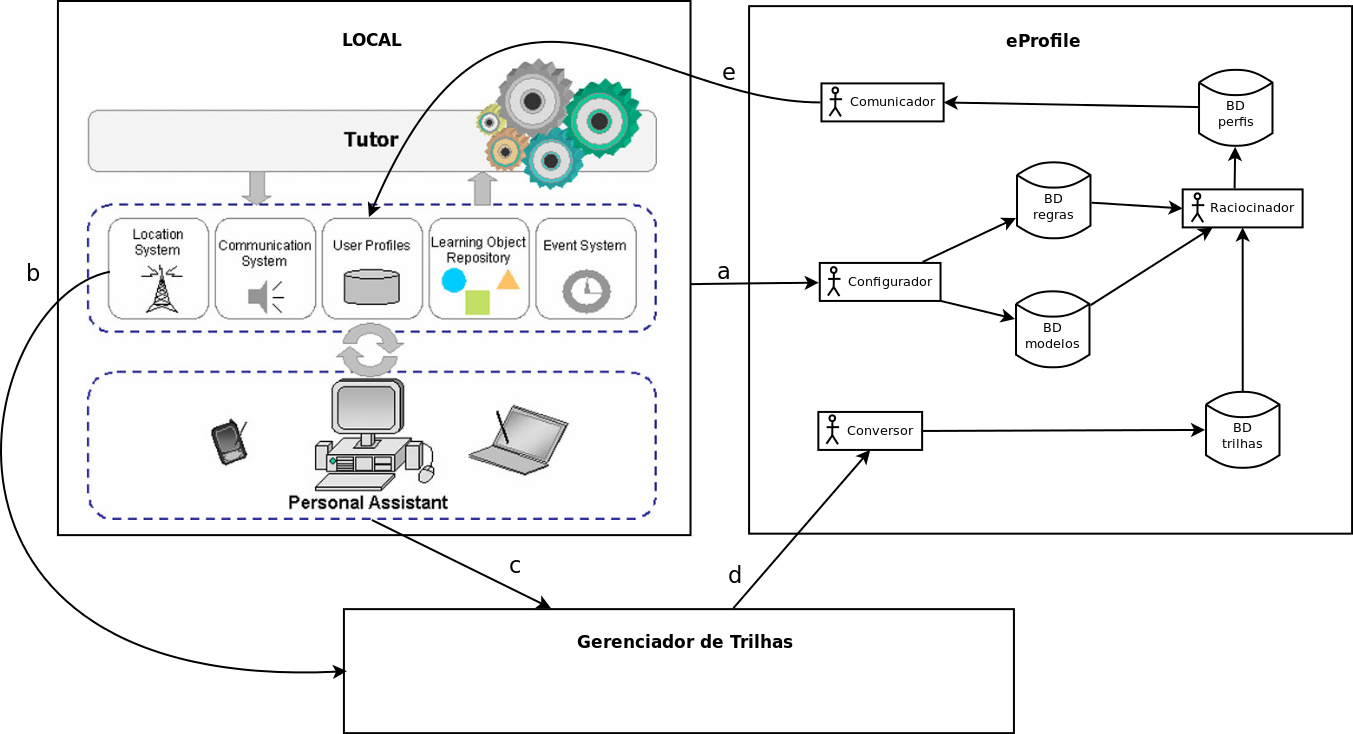
\includegraphics[width=1\textwidth]{../imagens/eprofile_local.png}
    \caption{Integração eProfile/LOCAL}
  \end{figure}
\end{frame}

%%%%%

\begin{frame}
  \frametitle{Cenário - Integração eProfile/UniManager}
  \begin{figure}[!t]
    \centering
\includegraphics[width=1\textwidth]{../imagens/unimanager_eprofile.png}
    \caption{Integração eProfile/UniManager}
  \end{figure}
\end{frame}

%%%%%

\begin{frame}
  \frametitle{Simulação do cenário}
  \begin{itemize}
    \item Início de semestre
      \begin{itemize}
        \item Alunos escolhem as disciplinas e se matriculam
        \item Cada dia é simulado, onde os alunos realizam debates, trabalhos e provas (14 aulas por semestre)
        \item A nota final dos alunos é calculada
      \end{itemize}
    \item Fim de semestre - continua?
  \end{itemize}
\end{frame}

%%%%%

\begin{frame}
  \frametitle{Regras, Trilhas e Perfis}
  \begin{itemize}
    \item Trilha contém escolhas feitas pelos estudantes (debates/trabalhos)
    \item Informações contextuais contém relações entre os assuntos
    \item Escolhas são vinculadas às relações entre os assuntos para obter o perfil
    \item Geração de perfil com interesses dos estudantes
      \begin{itemize}
        \item LOCAL: usa perfil para recomendar novos assuntos
        \item UniManager: usa perfil para recomendar disciplinas eletivas
      \end{itemize}
  \end{itemize}
\end{frame}

%%%%%

\begin{frame}
  \frametitle{Resultado}
  \begin{figure}[!t]
    \centering
\includegraphics[width=0.55\textwidth,angle=-90]{../imagens/auto.eps}
    \caption{Recomendações automáticas por semestre}
  \end{figure}
\end{frame}

%%%%%

\begin{frame}
  \frametitle{Avaliação 2 - alteração de regras}
  \begin{itemize}
    \item Diferencial do eProfile: alteração de regras durante a execução
    \item Nova regra: recomendação também ocorre baseada nas escolhas feitas pelos alunos mais ``semelhantes''
    \item Alunos ``semelhantes'' são os que fizeram as mesmas escolhas previamente
    \item Regra aplicada a partir do 7º semestre
  \end{itemize}
\end{frame}

%%%%%

\begin{frame}
  \frametitle{Resultado - Avaliação 2}
  \begin{figure}[!t]
    \centering
\includegraphics[width=0.55\textwidth,angle=-90]{../imagens/auto2.eps}
    \caption{Recomendações automáticas por semestre}
  \end{figure}
\end{frame}

%%%

\begin{frame}
  \huge Conclusão
\end{frame}

%%%%%

\begin{frame}
  \frametitle{Contribuições}
  \begin{itemize}
    \item Utilização de trilhas para extração de perfis
    \item Geração de perfis dinâmicos
    \item Gerenciamento {\em online} de regras de inferências e modelos de entidade dinâmicos 
    \item Interoperabilidade semântica
  \end{itemize}
\end{frame}

%%%%%%%%%%%%%%%%%%%%%%

\begin{frame}{Trabalhos relacionados}

	\begin{table}\centering\tiny
  \begin{tabular*}{1\textwidth}{@{}llllllllll@{}}
    \toprule
                              & PeLeP    & Chellouche & UUCM      & Kim       & Razmerita & Tao       & {\bf eProfile}  \\
    \midrule
    Interoperabilidade        & Não      & Sintática  & Sintática & Sintática & Sintática & Semântica & {\bf Semântica} \\
    Modelos dinâmicos         & Não      & Não        & Não       & Não       & Não       & Não       & {\bf Sim}       \\
    Armazenamento             & Servidor & Servidor   & Cliente   & Servidor  & Servidor  & Servidor  & {\bf Servidor} \\
    Sensibilidade a contexto  & Sim      & Sim        & Sim       & Não       & Sim  & Sim  & {\bf Sim} \\
    Utiliza trilhas           & Parcial  & Não        & Não       & Parcial   & Parcial   & Parcial   & {\bf Sim}      \\
    Domínio                   & Educação & Multimídia & Genérico  & Genérico  & Genérico  & Genérico  & {\bf Genérico} \\
    \bottomrule
  \end{tabular*}
  \caption{Comparação entre os trabalhos apresentados}
  \label{tab:comparacao}
\end{table}

\end{frame}

%%%%%

\begin{frame}
  \frametitle{Trabalhos futuros}
  \begin{itemize}
    \item Avaliação com entidades reais (não simuladas)
    \item Avaliação de desempenho
    \item Integração com outras aplicações em outros domínios
    \item Outros gerenciadores de trilhas
    \item Suporte à operação desconectada
    \item Descentralização do servidor
    \item Suporte a protocolos de segurança e confidencialidade
  \end{itemize}
\end{frame}

%%%%%

\begin{frame}
  \frametitle{Obrigado!}
  Perguntas?
\end{frame}

\end{document}
